%/////////////////////////////////////////////////////////%
%		   
% file: 	Report.tex
% version:	0.2 
% modified:	25 Mar 2015
% author:	David Bernard (bernardd@uvic.ca)
% descr:	A document that follows the University of Victoria
%			style guide for work term reports. The letter of
%			transmittal is included from a separately generated
%			pdf.
%
%/////////////////////////////////////////////////////////%

%%% To Do: More Package Cleanup
%			Margins
%	




%/////////////////////////////////////////////////////////%
%//						PREAMBLE						//%
%/////////////////////////////////////////////////////////%

\documentclass[12pt]{article}

%%%%%%%%%%%%%%%%%%%%%%%
% 	  Packages
%%%%%%%%%%%%%%%%%%%%%%%

% Math
\usepackage{
			amsmath,			% math operators
			amssymb,			% math symbols
			amsthm,				% theorem environment
			textcomp,			% Provides extra symbols
			xfrac				% diagonal fractions
			}

% Fonts
\usepackage[T1]{fontenc}		%better font encoding
\usepackage[utf8]{inputenc}		%better font encoding

%Graphics
\usepackage{
			graphicx,			% allow insertion of images
			tikz,				% vector graphics
			epstopdf,			% eps files
			pgfplots,			% plots in vector graphics
%			subfigure,			% allows subfigures (a), (b), etc.
			}
\pgfplotsset{compat=1.8}
			
%\usepackage[usenames,dvipsnames,svgnames,table]{xcolor}				% allow colour
	

% Tables					%%%%%%%%% Use Excel2LaTeX for easy table creation
\usepackage{
			tabularx,			%professional tables
			booktabs,
			multirow,
			bigstrut,
			diagbox,
			slashbox,
			}
%	\newcolumntype{Y}{>{\centering\arraybackslash}X}	%type Y - even column width - centered


% Formatting
\usepackage{
%			multicol,			% allow multi columns
%			parskip,			% disable indents
			relsize,			% for use with uppercase subscripts to make sizing more consistant
			pdfpages,			% import pdfs into this document
%			rotating,			% sideways figures
%			pdflscape, 			% allows landscape pages and rotates landscape pages in pdf file 
%			lscape,				% allows landscape pages
			framed,				% nice boxes; used in Supervisor's Approval
%			caption,			% line breaks in captions with \\
%			fancyhdr,			% see config in LAYOUT AND STYLING
%			lastpage,			% used with (fancyhdr)
			fullpage,			% set full page margins
			}
\usepackage[hidelinks]{hyperref}	%hyperlinks
	\hypersetup{
%   			colorlinks=false, 	%set true if you want colored links
				linktoc=all,     	%set to all if you want both sections and subsections linked
%    			linkcolor=blue,  	%choose some color if you want links to stand out
				}

% fancyhdr settings
%	\pagestyle{fancy}
%	\lhead{}
%	\chead{}
%	\rhead{}
%	\lfoot{}
%	\cfoot{\thepage}
%	\rfoot{}
%	\renewcommand{\headrulewidth}{0pt}
%	\renewcommand{\footrulewidth}{0pt}
	


% References
%\usepackage[sorting=none]{biblatex}
%\usepackage{csquotes}
%\bibliography{file}	%Bib File name

% Units
\usepackage{siunitx}
\usepackage{cancel}	%allows crossing out of units
	\sisetup{load-configurations = abbreviations}
	\sisetup{per-mode = fraction}
	%\sisetup{per-mode = symbol}
\usepackage[version=3]{mhchem}		%chemistry
	

% Misc				%%Figure out what these do
%\usepackage{enumerate}		
%\usepackage{nth}
%\usepackage{gensymb}
\usepackage{todonotes}	% To do notes
%\usepackage{capt-of}
%\usepackage{adjustbox}
%\usepackage{blindtext}


%%%%%%%%%%%%%%%%%%%%%%%
% Macros and Commands
%%%%%%%%%%%%%%%%%%%%%%%


%scientific notation  use \e
\providecommand{\e}[1]{\ensuremath{\times 10^{#1}}}

%diferential	use \d
%\def \d {\ensuremath{\mathrm{d}}}

%email
\newcommand{\email}[1]{\href{mailto:#1}{\texttt{#1}}}

%blank page
%\newcommand*\NewPage{\newpage\null\thispagestyle{empty}\newpage}

% for use with uppercase subscripts to make sizing more consistant
\newcommand{\s}[1]{_{\!\mathsmaller{#1}}}

% horizontal line for title page
\newcommand{\linia}{\rule{\linewidth}{0.5pt}}




%%%%%%%%%%%%%%%%%%%%%%%
% 	Environments
%%%%%%%%%%%%%%%%%%%%%%%

	
% Hides the formatting for the summary
\newenvironment{Summary}
	{ % beginning formatting
		% manually add entry to the toc since section*
		% suppresses addition to toc 
		\addcontentsline{toc}{section}{Summary}	
		\topskip 0pt				% remove top padding
		\vspace*{\stretch{2}}	% Pad 2/3 of the page length
		\section*{Summary}		% don't append a section number before "Summary"
	}
	{ % end formatting
		\vspace*{\stretch{3}}
	}

% Hides the formatting for the glossary
\newenvironment{Glossary}
	{ 	%beginning formatting
		\addcontentsline{toc}{section}{Glossary}	
 		\section*{Glossary}		
		\begin{description}
	}
	{
		\end{description}
	}


% Set up page numbering for appendices as (Appendix Letter) - (Page Number)
\providecommand{\StartAppendices}{
	\newpage
	\newcounter{AppendixCounter}	
	\renewcommand{\thepage}{\Alph{AppendixCounter} - \arabic{page}}
}

% Manually construct the section title for each appendix and then
% add an entry to the ToC 
\providecommand{\Appendix}[1]{
	\newpage
	\stepcounter{AppendixCounter}
	\setcounter{page}{1}
	\section*{Appendix \Alph{AppendixCounter}\quad #1}
	\addtocontents{toc}{\protect\contentsline{section}{Appendix \Alph{AppendixCounter}\quad #1}{}{}}
	% \protect preserves the spacing in the ToC
}




%/////////////////////////////////////////////////////////%
%//						BODY							//%
%/////////////////////////////////////////////////////////%

\begin{document}



%%%%%%%%%%%%%%%%%%%%%%%
% 	  Title Page
%%%%%%%%%%%%%%%%%%%%%%%


\begin{titlepage}
\newcommand{\HRule}{\rule{\linewidth}{0.5mm}} 
\center 

% Title Page Headings
\textsc{\LARGE University of Victoria}\\[0.25cm]
\textsc{\Large Faculty of Engineering}\\[0.5cm]
\textsc{\large TERM YEAR Work Term Report}\\[0.5cm] %date

\HRule \\[0.4cm]
{ \huge \bfseries TITLE}\\ % Document Title
\HRule \\[1 cm]
 
\begin{center}\large
Department of Mechanical Engineering\\
University of Victoria\\
Victoria, BC\\[1cm]

First \textsc{Last}	\\ %your name
V0011111111	\\
Work Term ?	\\
Mechanical Engineering\\
\email{email@uvic.ca}\\[1cm]
\end{center}


{\large \today}\\[0.5cm] % Date


\includegraphics{UVic_logo}\\[0.5cm]


\noindent\makebox[\textwidth][c]{
	\begin{minipage}{1.1\textwidth}
		\begin{flushleft}
			\begin{framed}
				\textbf{Supervisor's Approval: To be completed by Employer}	\\
				I approve the release of this report to the University of Victoria for evaluation purposes only.\\
				The report is to be considered (select one): $ \square $ NOT CONFIDENTIAL $ \square $ CONFIDENTIAL\\
				\vspace{.25cm}
				Signature: \underline{\hspace{4.3 cm}} Position: \underline{\hspace{4 cm}}  Date: \underline{\hspace{3 cm}} \\
				\vspace{.25cm}
				Name (print): \underline{\hspace{4 cm}} E-Mail: \underline{\hspace{4 cm}} Fax : \underline{\hspace{3 cm}} \\
				If a report is deemed CONFIDENTIAL, a non-disclosure form signed by an evaluator will be faxed to the employer. The report will be destroyed following evaluation. If the report is NOT
				CONFIDENTIAL, it will be returned to the student following evaluation.
			\end{framed}
		\end{flushleft}
	\end{minipage}
}




\end{titlepage}





%\NewPage %blank added for double sided printing


%%%%%%%%%%%%%%%%%%%%%%%
% Letter of Transmittal
%%%%%%%%%%%%%%%%%%%%%%%
\clearpage

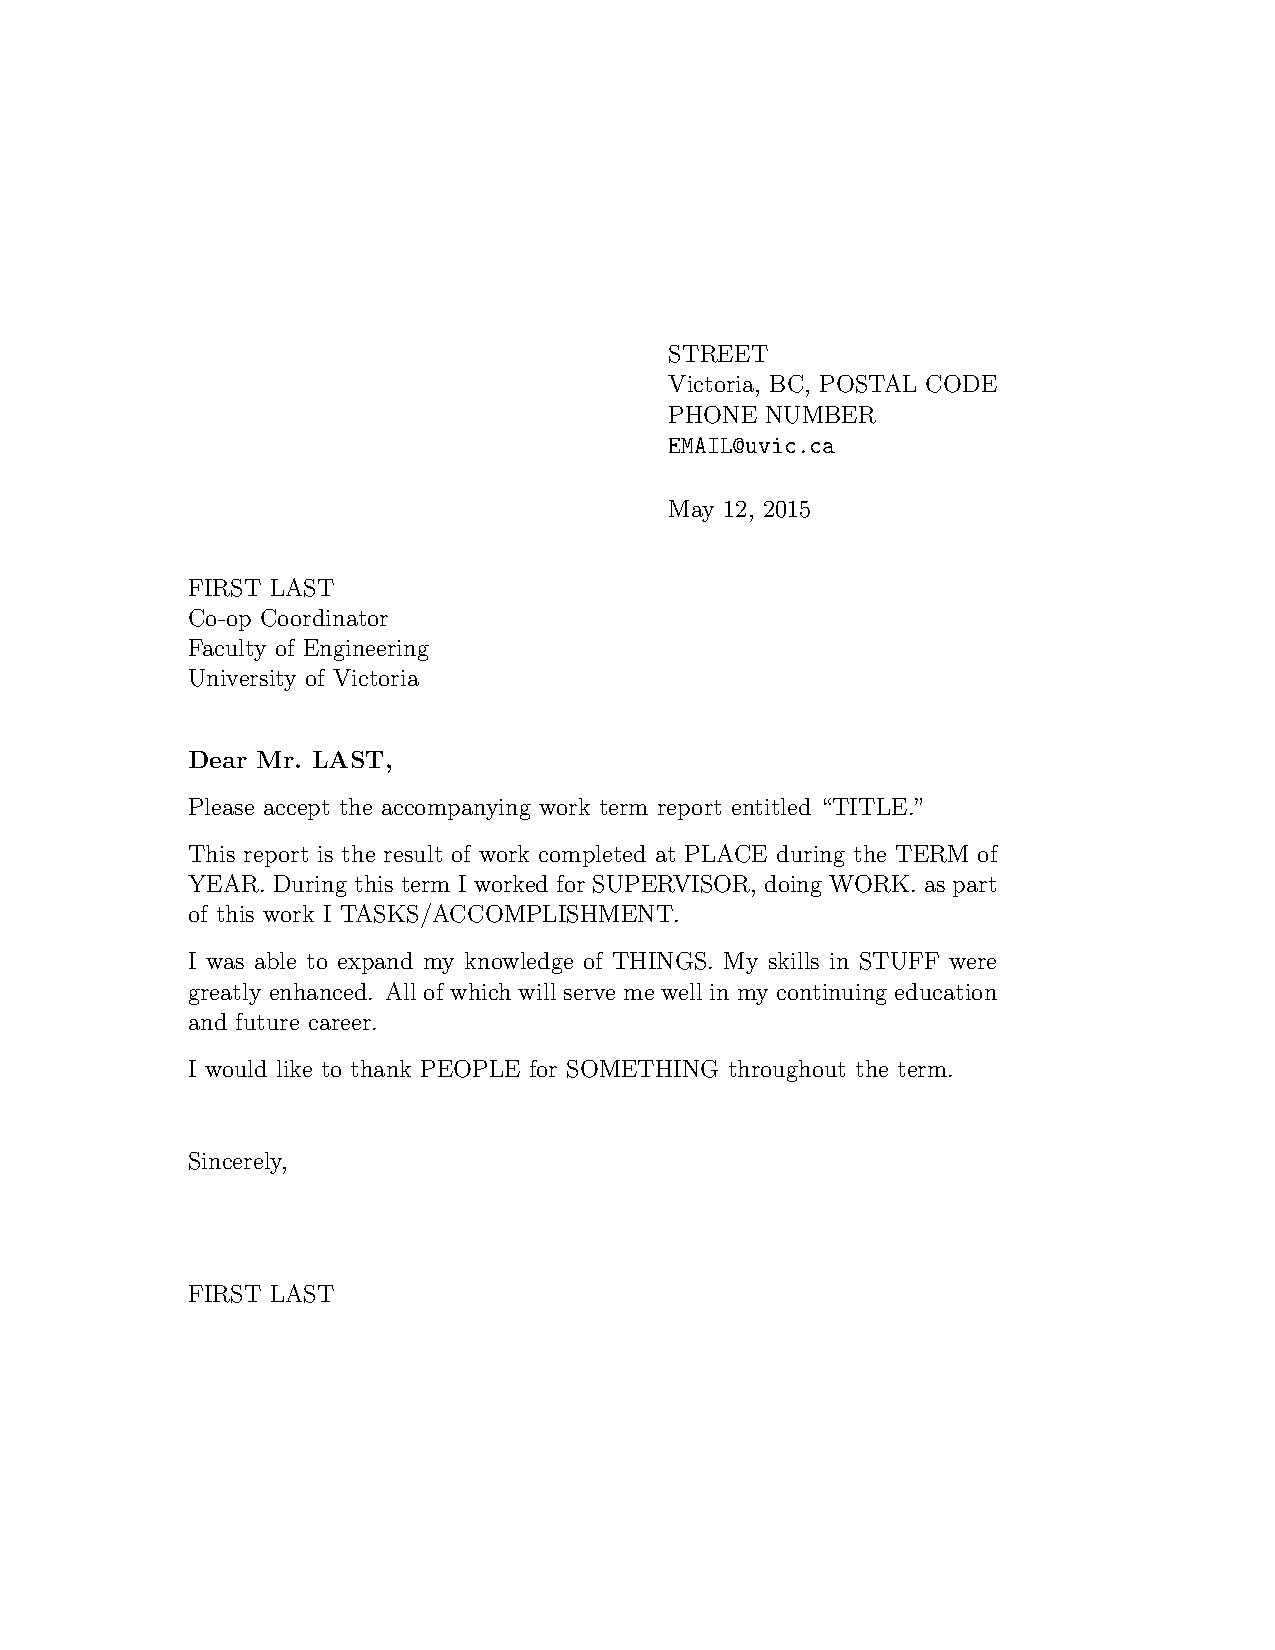
\includepdf[]{./Letter/letter.pdf}


%%%%%%%%%%%%%%%%%%%%%%%
%  Tables of Contents
%%%%%%%%%%%%%%%%%%%%%%%

\pagenumbering{roman}
%\setcounter{page}{1}
\tableofcontents



\cleardoublepage
%\phantomsection

\listoffigures \addcontentsline{toc}{section}{\listfigurename}

\pagebreak


%%%%%%%%%%%%%%%%%%%%%%%
% 		Summary
%%%%%%%%%%%%%%%%%%%%%%%


\begin{Summary}
The summary is written for the general reader who wishes to be familiar with the content of the report while avoiding details. The summary is a separate report, stating the engineering problem, the approach to the solution, the main conclusions and recommendations. It is written after the main report has been completed. Items in the main report such as tables, figures or sections, are not referred to in the summary. The summary is normally presented centered on its own page, and is less than one page in length.
\end{Summary}









%\section*{Summary} \addcontentsline{toc}{section}{Summary}

\pagebreak


%%%%%%%%%%%%%%%%%%%%%%%
% 		Glossary
%%%%%%%%%%%%%%%%%%%%%%%

\begin{Glossary}
	\item[Uvic] University of Victoria
\end{Glossary}


%\section*{Glossary} \addcontentsline{toc}{section}{Glossary}

\newpage



%%%%%%%%%%%%%%%%%%%%%%%%%%%%%%%%%%%%%%%%%%%%%%%
%%%%          Document Starts Here      %%%%%%%



\pagenumbering{arabic}
\section{Introduction}

\newpage

\section{Discussion}




\section{Conclusions}

\section{Recommendations}


	\begin{table} [h]
		content...
		\caption{tab 1}
	\end{table}

	\begin{figure} [h]
		\caption{fig 1}
	\end{figure}
	
\pagebreak



%%%%%%%%%%%%%%%%%%%%%%%
% 	  Referrences
%%%%%%%%%%%%%%%%%%%%%%%
\pagebreak
\addcontentsline{toc}{section}{References}

references here
%\bibliographystyle{ieeetr}
%\bibliography{wt_template}
% Update entries in bibdesk using texshop to typeset
% typsetting: 1) latex 2) bibdesk 3) latex 4) latex




%%%%%%%%%%%%%%%%%%%%%%%
% 	   Appendices
%%%%%%%%%%%%%%%%%%%%%%%

\StartAppendices

\Appendix{My appendix}
Here is some text for my appendix.

\Appendix{Appendix 2}
new text

\end{document}